\documentclass{beamer}
\usetheme{Dresden}
%\usetheme{CambridgeUS}
\usepackage{helvet}
\usepackage{cite}
\usepackage{url}
\usepackage{amssymb, amsmath, graphicx, charter, latexsym}
\usepackage{subfigure}
\usepackage{enumerate}
\usepackage{ragged2e}
\usepackage{mathtools}
\usepackage{tabu}
\usepackage{epstopdf}
\usepackage{siunitx}
\usepackage{calligra}
\usepackage{listings}
\usepackage{todonotes}
\renewcommand{\familydefault}{\sfdefault}
%\usepackage{times}

\setbeamertemplate{items}[circle]
\setbeamertemplate{navigation symbols}{}
\setbeamertemplate{caption}{\insertcaption}

\newcommand{\argmax}{\operatorname{argmax}}
\lstset{
basicstyle=\ttfamily,
}

\begin{document}
\title{S-WiFi: Smart Scheduling with Point Coordination Function for WiFi Uplink}
\author{Dongni Han, Ping-Chun Hsieh, and Tao Zhao}
\date{April 28, 2016}
\newtheorem{thm}{Theorem}
\begin{frame}
\titlepage
\end{frame}


%\begin{frame}
%\frametitle{What to Discuss Today?}
%\tableofcontents[]
%\end{frame}

%\AtBeginSection[]
%{
	%\begin{frame}{Table of Contents}
	%\tableofcontents[currentsection]
	%\end{frame}
%}

\NewDocumentCommand{\varSI}{O{}}{\SI[detect-all=true,parse-numbers=false,#1]}

\section{Background}

\begin{frame}
\frametitle{System Model}
\begin{itemize}
  \item WiFi network
    \begin{itemize}
      \item One AP and $N$ clients
      % \varSI must be outside math env for it to have right font family.
      \item Time slotted; $\SI{1}{interval} =$ \varSI{T}{slots}
    \end{itemize}
  \item Uplink
    \begin{itemize}
      \item Packets generated by each client $n$ in each interval
      \item Number of packets $X_n$ follows Unif$\{U_\text{min}, U_\text{max}\}$
      \item Real-time traffic
    \end{itemize}
  \item Point Coordination Function (PCF)
    \begin{itemize}
      \item AP polls (at most) one client per slot
      \item But AP needs to know $X_n$ first!
    \end{itemize}
\end{itemize}
\end{frame}

\begin{frame}
\frametitle{Baseline Policy: Phase 1}
\begin{itemize}
\item AP polls $X_n$ for all $n$ one by one
\end{itemize}
\begin{figure}
\centering
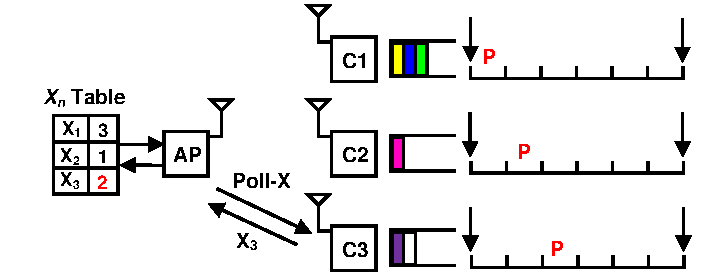
\includegraphics[scale=0.8]{animation_03.pdf}
\end{figure}
\end{frame}

\begin{frame}
\frametitle{Baseline Policy: Phase 2}
\begin{itemize}
\item AP uses Max-Weight scheduling for data transmissions
\end{itemize}
\begin{figure}
\centering
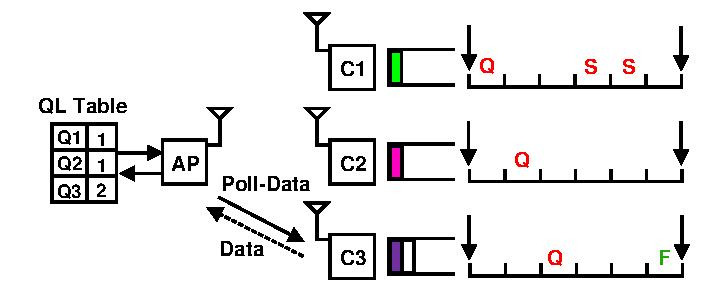
\includegraphics[scale=0.8]{animation_06.pdf}
\end{figure}
\end{frame}

\begin{frame}{Baseline Policy: Issues}
  \begin{itemize}
    \item No data transmissions in Phase 1
    \item Channel utilization for data packets is low
    \item Huge overhead especially with large $N$ and poor channel
      \pause
    \item We need a smart policy!
  \end{itemize}
\end{frame}
\section{Smart Policy}

\begin{frame}
\frametitle{Idea 1: Selective Polling}
\begin{itemize}
\item Only poll $n \le N$ clients per interval
\item Random permutation for fairness
\item Consider remaining clients only after all selected are served
\end{itemize}
\begin{figure}
\centering
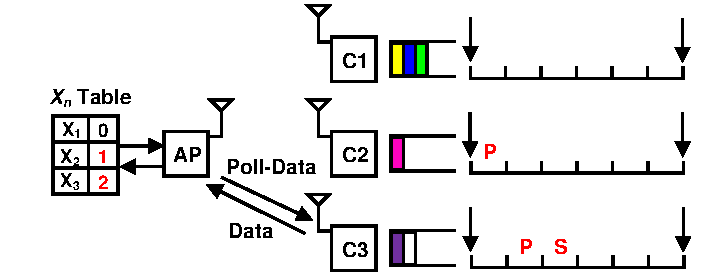
\includegraphics[scale=0.8]{selective_1.pdf}
\caption{Example: $n=2, N=3$}
\end{figure}
\end{frame}

\begin{frame}
\frametitle{Feature 001: Selective Polling}
\begin{itemize}
\item How to determine the optimal $n$?
  \begin{itemize}
    \item Sort clients by channel reliabilities $p_1 > p_2 > \dots > p_N$
    \item Estimated throughput: $\hat{R}_n = \min\{n\overline{U}, (T-\sum_{i=1}^{n}\frac{1}{p_i})\frac{\sum_{i=1}^{n}p_i}{n} \}$
    \item Find the optimum $n^* = \argmax_{n} \hat{R}_n$
  \end{itemize}
\item Random permutation?
  \begin{itemize}
    \item Classic problem: Knuth shuffle algorithm
  \end{itemize}
\item How to schedule remaining clients?
  \begin{itemize}
    \item Serve the clients one by one
  \end{itemize}
\end{itemize}
\end{frame}

\begin{frame}
\frametitle{Idea 2: Piggybacked Queue Length}
\begin{itemize}
\item Client replies in one packet
  \begin{itemize}
    \item $X_n$
    \item first data message if $X_n>0$
  \end{itemize}
\end{itemize}
\begin{figure}
\centering
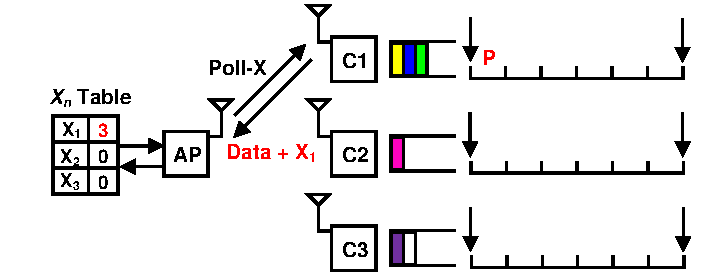
\includegraphics[scale=0.8]{piggyback_1.pdf}
\end{figure}
\end{frame}

\begin{frame}
\frametitle{Feature 010: Piggybacking}
\begin{itemize}
  \item New packet types
    \begin{itemize}
      \item \lstinline|SWiFi_PKT_POLL_PGBK|
      \item \lstinline|SWiFi_PKT_PGBK_UL|
    \end{itemize}
  \item If combined with selective polling
    \begin{itemize}
      \item All slots are effectively available for data
      \item Estimated throughput: $\hat{R}_n = \min\{n\overline{U}, \alert{T}\frac{\sum_{i=1}^{n}p_i}{n} \}$
    \end{itemize}
\end{itemize}
\end{frame}

\begin{frame}
\frametitle{Idea 3: Retry Limit for Polling}
\begin{itemize}
\item Avoid spending too much time on clients with poor channel
\end{itemize}
\begin{figure}
\centering
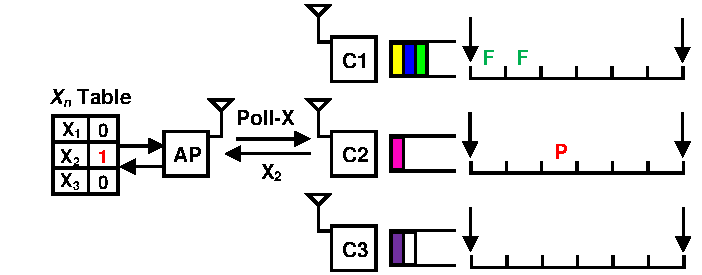
\includegraphics[scale=0.8]{retry_1.pdf}
\caption{Example: $p_1=0.1$, retry limit $= 1$}
\end{figure}
\end{frame}

\begin{frame}
\frametitle{Feature 100: Retry Limit}
\begin{itemize}
  \item Set \lstinline|num_retry_ = 0| for the newly polled client
  \item If retry limit reached: poll the next client in the next slot
    regardless the last transmission is successful or not
  \item Otherwise: \lstinline|num_retry_++|
\end{itemize}
\end{frame}

\begin{frame}{Feature 111: Our Smart Policy}
  \begin{itemize}
    \item Selective Polling + Piggybacking + Retry Limit
      \begin{itemize}
	\item Select a subset of clients to poll $X_n$
	\item AP polls clients in expect of piggybacking reply
	\item AP repeats polling a client for limited times
      \end{itemize}
    \item All combinations of three features are possible
      \begin{itemize}
	\item Special case: baseline $=$ 000
      \end{itemize}
  \end{itemize}
\end{frame}

\section{Simulation}
\begin{frame}{Simulation Setup}
  \begin{itemize}
    \item $\SI{1}{slot} = \SI{10}{ms}, T=10$
    \item Number of clients $N=5$
    \item Number of packets $U_\text{min}=0, U_\text{max}=2$
    \item Channel reliability $p\approx0.57$ (distance \SI{1000}{m})
    \item Retry limit: 1
    \item Metric: total timely-throughput of all clients
      \begin{itemize}
	\item Averaged over 10 runs
      \end{itemize}
  \end{itemize}
\end{frame}
%\begin{frame}
%\frametitle{Simulation Results: Network Capacity}
%\begin{itemize}
%\item $N=2$ and $T=10$
%\item Reliable channel: $p_1 = p_2 = 1$ (symmetric)
%\item $N_\text{max}$ ranges from $1$ to $20$
%\item Real-time traffic
%\end{itemize}
%\begin{figure}
%\centering
%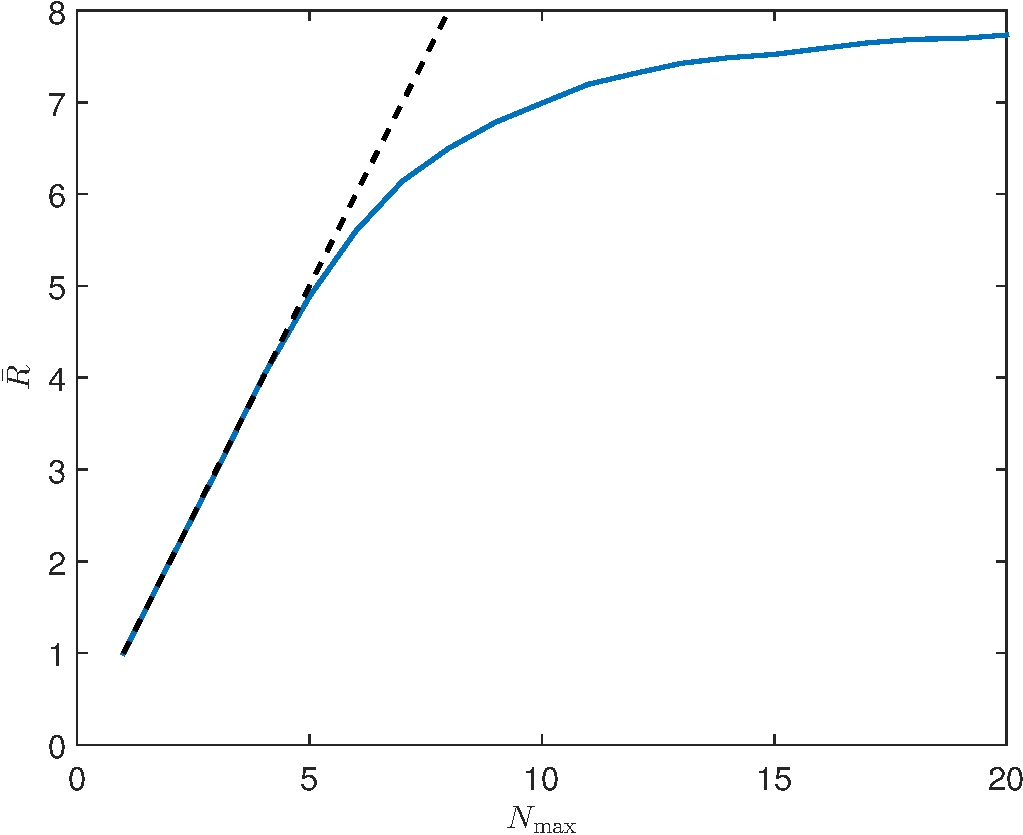
\includegraphics[height=.5\textheight]{realtime_throughput_randmax.pdf}
%\caption{Packet deadline reduces the capacity further.}
%\end{figure}
%\end{frame}

\begin{frame}
\frametitle{Performance under Symmetric Channel}
\begin{columns}
  \begin{column}{.5\textwidth}
    \begin{itemize}
      \item Symmetry: $p_i=p, i=1,2,\dotsc,N$
      \item $p$ ranges from $0$ to $1$
      \item Smart is always better
      \item Huge improvement when the channel reliability is moderate
      \item Smart delivers all packets when $p=1$
    \end{itemize}
  \end{column}
  \begin{column}{.5\textwidth}
    \begin{figure}[htbp]
      \centering
      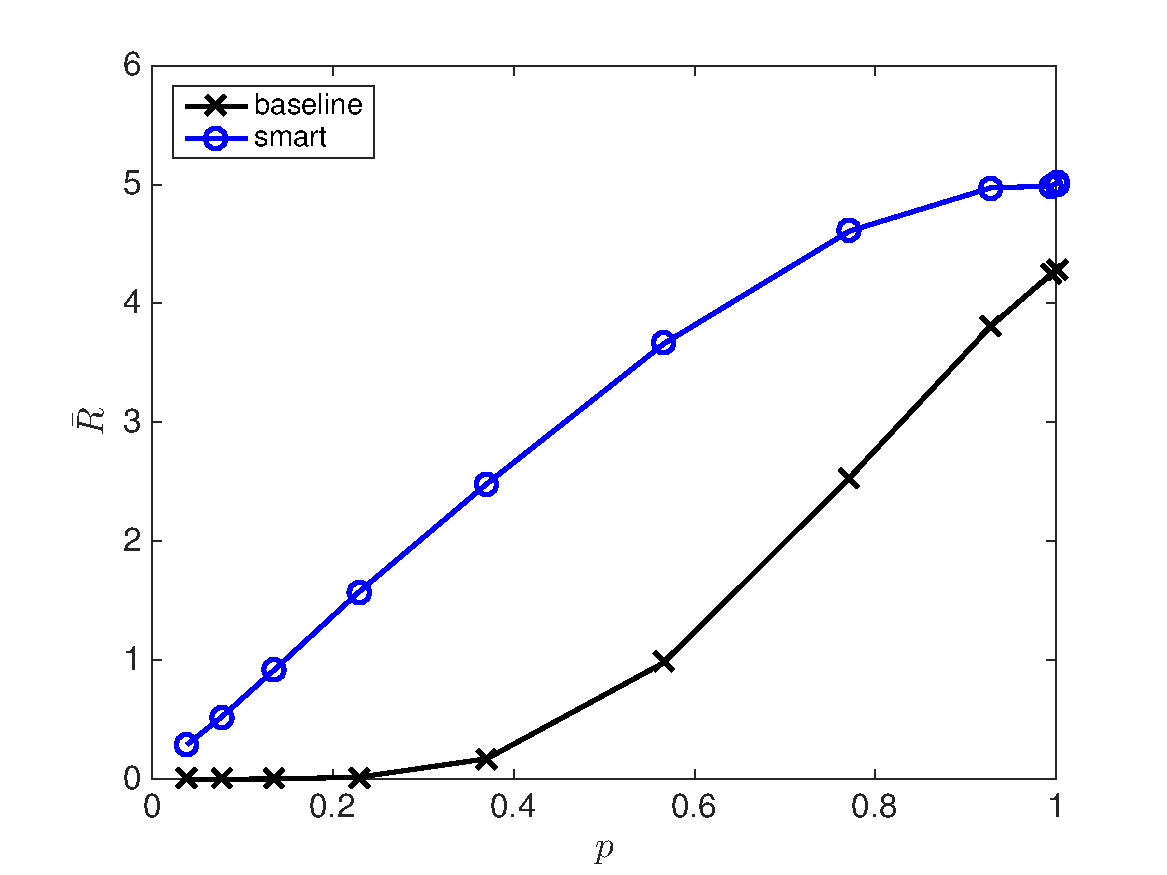
\includegraphics[height=.5\textheight]{R_p_sym.pdf}
      \caption{Throughout v.s. channel reliability.}
    \end{figure}
  \end{column}
\end{columns}
\end{frame}

\begin{frame}
\frametitle{Impact of Number of Clients}
\begin{columns}
  \begin{column}{.5\textwidth}
\begin{itemize}
\item $N$ ranges from $2$ to $10$
\item Symmetric channel
\item Smart is better in general.
  \begin{itemize}
    \item The case with $N=2$ is due to retry limit $=1$.
  \end{itemize}
\item As $N$ goes very large, Baseline gives $0$ throughput while Smart
  performs steadily.
\end{itemize}
  \end{column}
  \begin{column}{.5\textwidth}
\begin{figure}[htbp]
  \centering
  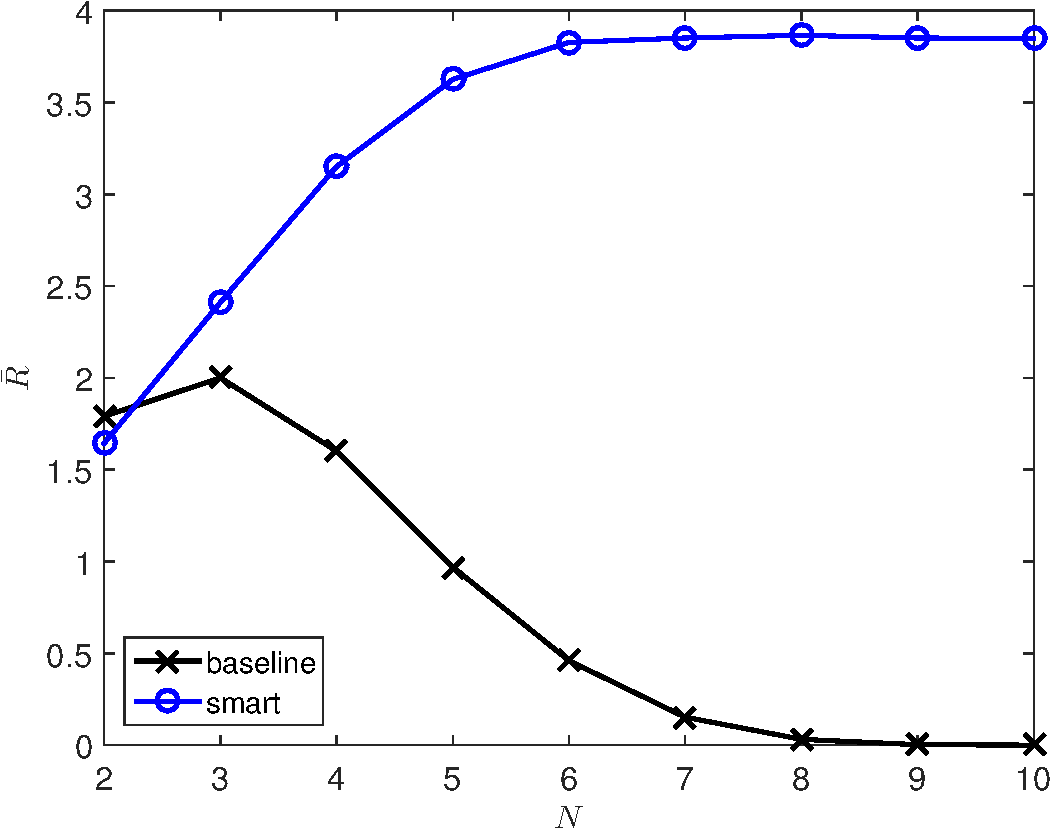
\includegraphics[height=.5\textheight]{R_N_sym.pdf}
  \caption{Throughout v.s. number of clients.}
\end{figure}
  \end{column}
\end{columns}
\end{frame}

\begin{frame}
\frametitle{Performance under Asymmetric Channel}
\begin{columns}
  \begin{column}{.5\textwidth}
\begin{itemize}
  \item Asymmetry
    \begin{itemize}
      \item $p_1=p_2=1$
      \item $p_j=p, j=3,4,\dotsc,N$
    \end{itemize}
  \item $p$ ranges from $0$ to $1$
  \item Smart is consistently better, especially when channel is poor
\end{itemize}
  \end{column}
  \begin{column}{.5\textwidth}
\begin{figure}[htbp]
  \centering
  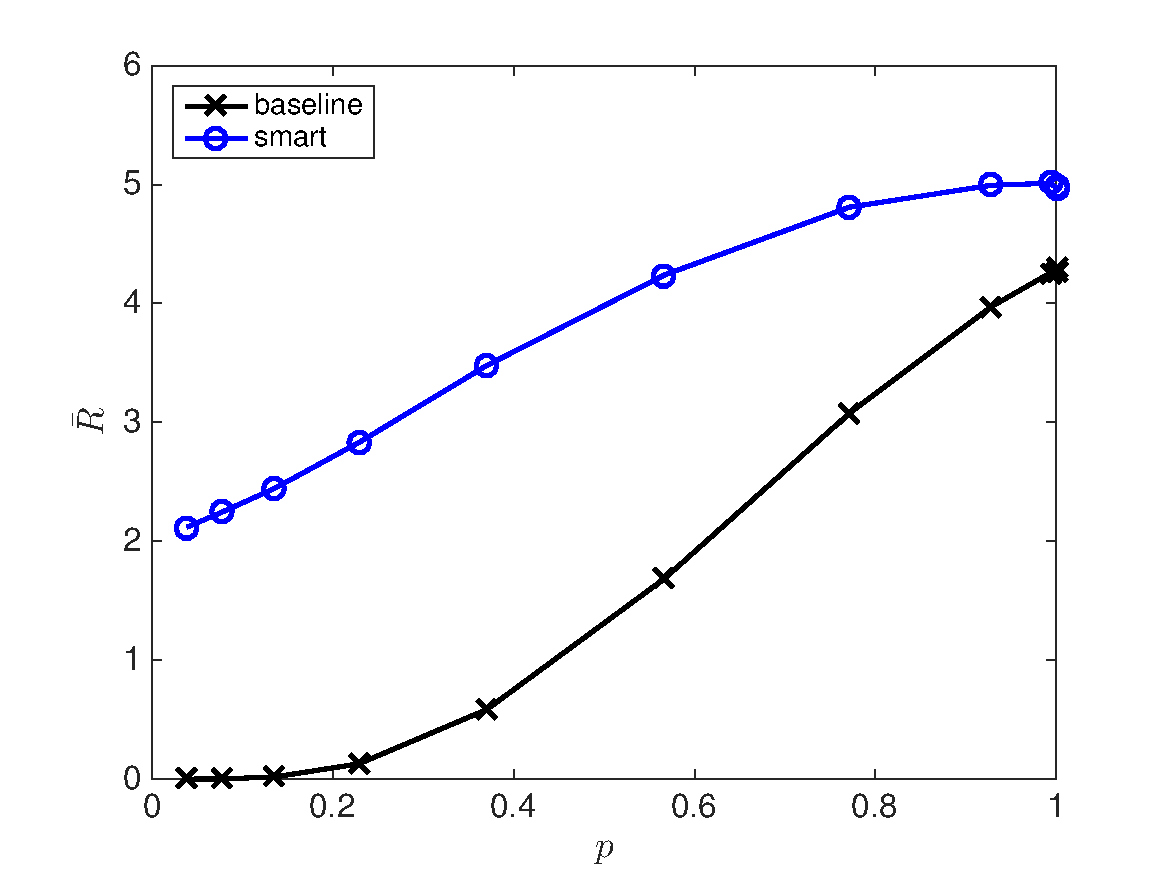
\includegraphics[height=.5\textheight]{R_p_asym.pdf}
  \caption{Throughout v.s. channel reliability of distant clients.}
\end{figure}
  \end{column}
\end{columns}
\end{frame}

%\begin{frame}{Network Utility}
%\begin{columns}
  %\begin{column}{.5\textwidth}
  %\begin{itemize}
    %\item $q_n$: timely-throughput for $n$
    %%\item $U_n(q_n) = \log (\frac{q_n}{10^{-4}})$
    %\item Network utility $\sum U_n(q_n) = \sum \log (\frac{q_n}{10^{-4}})$
    %\item Symmetric channel
    %\item Smart is also much better in terms of network utility
      %regardless of channel reliabilities.
    %\item Utility of Baseline is $-\infty$ with poor channel.
  %\end{itemize}
  %\end{column}
  %\begin{column}{.5\textwidth}
%\begin{figure}[htbp]
  %\centering
  %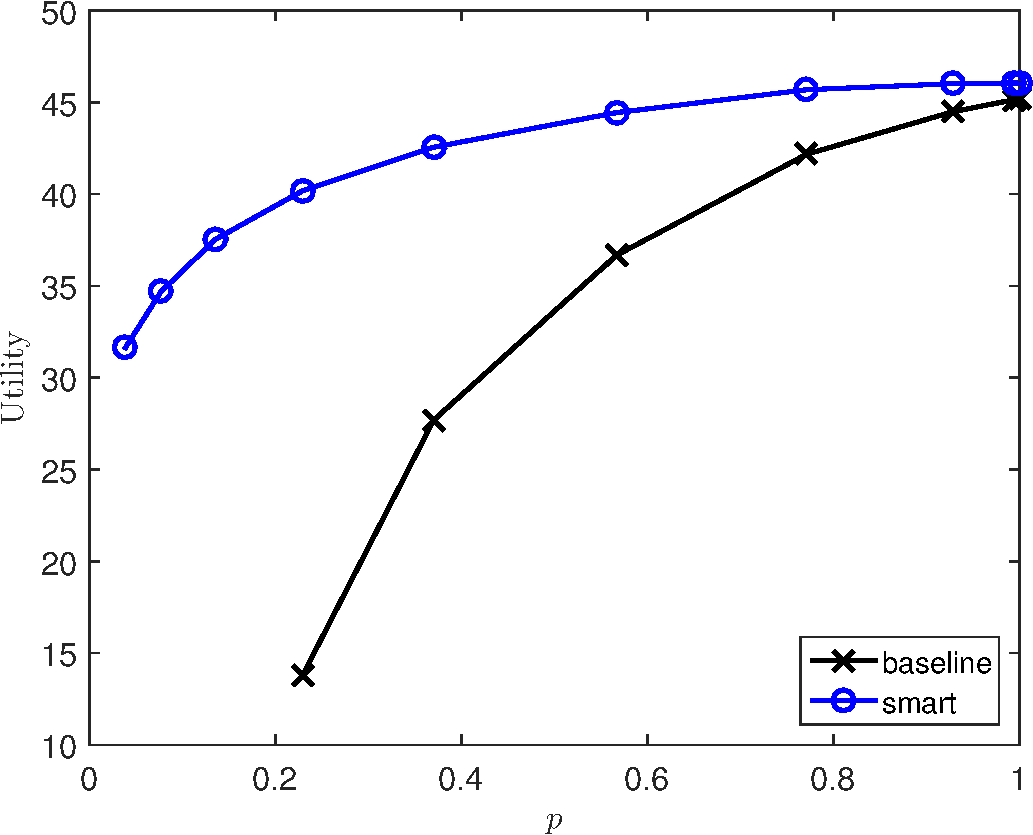
\includegraphics[height=.5\textheight]{U_p_sym.pdf}
  %\caption{Utility v.s. channel reliability.}
%\end{figure}
  %\end{column}
%\end{columns}
%\end{frame}

\begin{frame}{Network Utility}
\begin{columns}
  \begin{column}{.5\textwidth}
  \begin{itemize}
    \item $q_n$: timely-throughput for $n$
    %\item $U_n(q_n) = \log (\frac{q_n}{10^{-4}})$
    \item Network utility $\sum U_n(q_n) = \sum \log (\frac{q_n}{10^{-4}})$
    \item Asymmetric channel
    \item Smart is also much better in terms of network utility
      regardless of channel reliabilities.
    \item Utility of Baseline is $-\infty$ with poor channel.
  \end{itemize}
  \end{column}
  \begin{column}{.5\textwidth}
\begin{figure}[htbp]
  \centering
  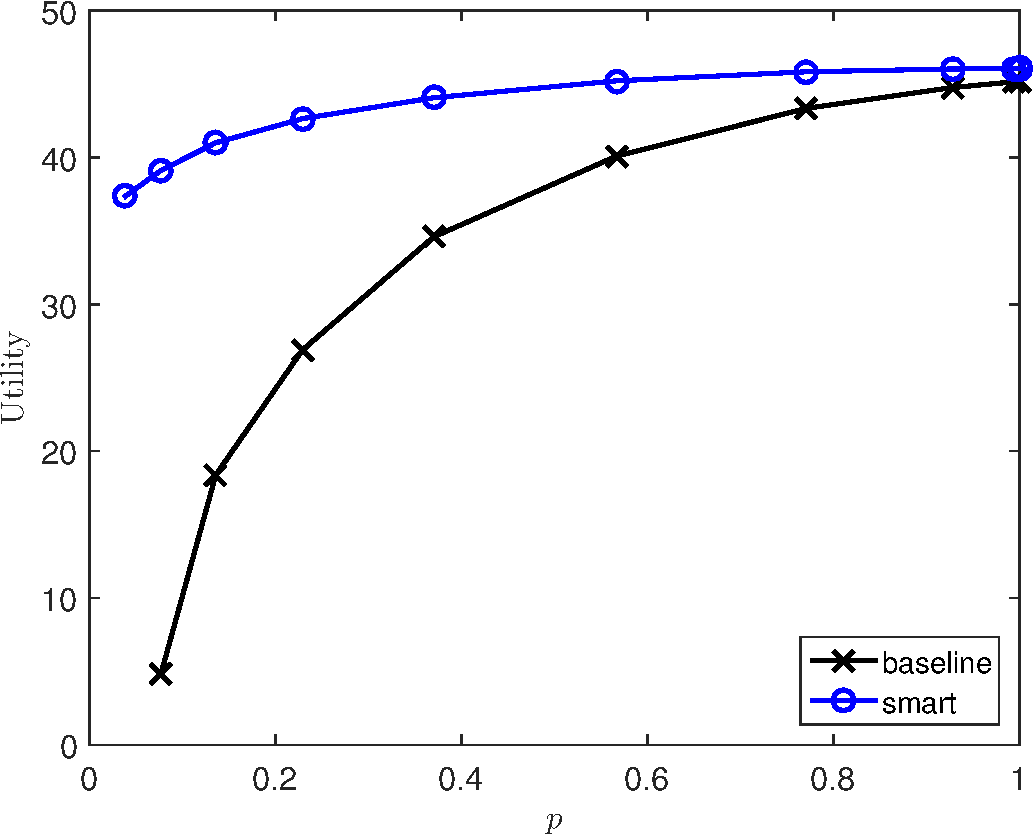
\includegraphics[height=.5\textheight]{U_p_asym.pdf}
  \caption{Utility v.s. channel reliability.}
\end{figure}
  \end{column}
\end{columns}
\end{frame}

\section*{Conclusion}
\begin{frame}{Conclusion}
  \begin{itemize}
    \item The baseline policy incurs huge overhead especially with large $N$ and poor channel.
    \item Our smart policy incoporates selective polling, piggybacking, and
      retry limit to improve the performance.
    \item Simulation shows our smart policy outperforms the baseline policy in
      terms of timely-throughput and network utility.
  \end{itemize}
\end{frame}

\begin{frame}{Outlook}
  \begin{itemize}
    \item Selective polling: weighted random permutation
    \item Retry limit: determine optimum automatically
    \item Phase 2: Debt based policies
    \item S-WiFi website, etc.
  \end{itemize}
\end{frame}

\begin{frame}
  \begin{center}
    {\Huge\calligra Thank you!}
  \end{center}
  \begin{figure}[htbp]
    \centering
    \includegraphics[height=.3\textheight]{qrcode.png}
  \end{figure}
\end{frame}
\end{document}
